% % % % % % % % % % % % % % % % % % % % % % % % % % % % % % % % % % % % % % % %
% IEEE Style - Double columns, 11pt font, letterpaper
\documentclass[journal, twocolumn, final,11pt,letterpaper]{IEEEtran}	

% Include Latex Packages
\usepackage{etex}	% This package enables the use of many packages

% % Page styles
\usepackage{setspace}	% line spacing package
\doublespacing			% use double spacing
%\linespread{1.6}		% Use linespread to fine tune line spacing, not recommended


% % Figures
\usepackage{float}		% improves interface for floating objects
\usepackage{subfig}		% enables subfloat
\usepackage{graphicx}	% more image type support
\usepackage{circuitikz}
\usepackage{epstopdf}	% automatically convert included eps files to pdf
\usepackage{tikz}
%\usepackage{listings}
\usepackage{color}
\definecolor{dkgreen}{rgb}{0,0.6,0}
\definecolor{gray}{rgb}{0.5,0.5,0.5}
\definecolor{mauve}{rgb}{0.58,0,0.82}

\lstset{frame=tb,
	language=Verilog,
	aboveskip=3mm,
	belowskip=3mm,
	showstringspaces=false,
	columns=flexible,
	basicstyle={\small\ttfamily},
	numbers=none,
	numberstyle=\tiny\color{gray},
	keywordstyle=\color{blue},
	commentstyle=\color{dkgreen},
	stringstyle=\color{mauve},
	breaklines=true,
	breakatwhitespace=true,
	tabsize=3
}
\usetikzlibrary{matrix,calc}
\usetikzlibrary{shapes}

\newcommand*{\circled}[2][red]{
	\tikz[baseline=(char.base)]{
		\node[shape=ellipse,inner sep=1pt,
		draw=#1,
		] (char) {#2};}
}

%isolated term
%#1 - Optional. Space between node and grouping line. Default=0
%#2 - node
%#3 - filling color
\newcommand{\implicantsol}[3][0]{
	\draw[rounded corners=3pt, fill=#3, opacity=0.3] ($(#2.north west)+(135:#1)$) rectangle ($(#2.south east)+(-45:#1)$);
}


%internal group
%#1 - Optional. Space between node and grouping line. Default=0
%#2 - top left node
%#3 - bottom right node
%#4 - filling color
\newcommand{\implicant}[4][0]{
	\draw[rounded corners=3pt, fill=#4, opacity=0.3] ($(#2.north west)+(135:#1)$) rectangle ($(#3.south east)+(-45:#1)$);
}

%group lateral borders
%#1 - Optional. Space between node and grouping line. Default=0
%#2 - top left node
%#3 - bottom right node
%#4 - filling color
\newcommand{\implicantcostats}[4][0]{
	\draw[rounded corners=3pt, fill=#4, opacity=0.3] ($(rf.east |- #2.north)+(90:#1)$)-| ($(#2.east)+(0:#1)$) |- ($(rf.east |- #3.south)+(-90:#1)$);
	\draw[rounded corners=3pt, fill=#4, opacity=0.3] ($(cf.west |- #2.north)+(90:#1)$) -| ($(#3.west)+(180:#1)$) |- ($(cf.west |- #3.south)+(-90:#1)$);
}

%group top-bottom borders
%#1 - Optional. Space between node and grouping line. Default=0
%#2 - top left node
%#3 - bottom right node
%#4 - filling color
\newcommand{\implicantdaltbaix}[4][0]{
	\draw[rounded corners=3pt, fill=#4, opacity=0.3] ($(cf.south -| #2.west)+(180:#1)$) |- ($(#2.south)+(-90:#1)$) -| ($(cf.south -| #3.east)+(0:#1)$);
	\draw[rounded corners=3pt, fill=#4, opacity=0.3] ($(rf.north -| #2.west)+(180:#1)$) |- ($(#3.north)+(90:#1)$) -| ($(rf.north -| #3.east)+(0:#1)$);
}

%group corners
%#1 - Optional. Space between node and grouping line. Default=0
%#2 - filling color
\newcommand{\implicantcantons}[2][0]{
	\draw[rounded corners=3pt, opacity=.3] ($(rf.east |- 0.south)+(-90:#1)$) -| ($(0.east |- cf.south)+(0:#1)$);
	\draw[rounded corners=3pt, opacity=.3] ($(rf.east |- 8.north)+(90:#1)$) -| ($(8.east |- rf.north)+(0:#1)$);
	\draw[rounded corners=3pt, opacity=.3] ($(cf.west |- 2.south)+(-90:#1)$) -| ($(2.west |- cf.south)+(180:#1)$);
	\draw[rounded corners=3pt, opacity=.3] ($(cf.west |- 10.north)+(90:#1)$) -| ($(10.west |- rf.north)+(180:#1)$);
	\fill[rounded corners=3pt, fill=#2, opacity=.3] ($(rf.east |- 0.south)+(-90:#1)$) -|  ($(0.east |- cf.south)+(0:#1)$) [sharp corners] ($(rf.east |- 0.south)+(-90:#1)$) |-  ($(0.east |- cf.south)+(0:#1)$) ;
	\fill[rounded corners=3pt, fill=#2, opacity=.3] ($(rf.east |- 8.north)+(90:#1)$) -| ($(8.east |- rf.north)+(0:#1)$) [sharp corners] ($(rf.east |- 8.north)+(90:#1)$) |- ($(8.east |- rf.north)+(0:#1)$) ;
	\fill[rounded corners=3pt, fill=#2, opacity=.3] ($(cf.west |- 2.south)+(-90:#1)$) -| ($(2.west |- cf.south)+(180:#1)$) [sharp corners]($(cf.west |- 2.south)+(-90:#1)$) |- ($(2.west |- cf.south)+(180:#1)$) ;
	\fill[rounded corners=3pt, fill=#2, opacity=.3] ($(cf.west |- 10.north)+(90:#1)$) -| ($(10.west |- rf.north)+(180:#1)$) [sharp corners] ($(cf.west |- 10.north)+(90:#1)$) |- ($(10.west |- rf.north)+(180:#1)$) ;
}

%Empty Karnaugh map 4x4
\newenvironment{Karnaugh}%
{
	\begin{tikzpicture}[baseline=(current bounding box.north),scale=0.8]
	\draw (0,0) grid (4,4);
	\draw (0,4) -- node [pos=0.9,above right,anchor=south west] {C1C0} node [pos=0.9,below left,anchor=north east] {EQ} ++(135:1);
	%
	\matrix (mapa) [matrix of nodes,
	column sep={0.8cm,between origins},
	row sep={0.8cm,between origins},
	every node/.style={minimum size=0.3mm},
	anchor=8.center,
	ampersand replacement=\&] at (0.5,0.5)
	{
		\& |(c00)| 00         \& |(c01)| 01         \& |(c11)| 11         \& |(c10)| 10         \& |(cf)| \phantom{00} \\
		|(r00)| 00             \& |(0)|  \phantom{0} \& |(1)|  \phantom{0} \& |(3)|  \phantom{0} \& |(2)|  \phantom{0} \&                     \\
		|(r01)| 01             \& |(4)|  \phantom{0} \& |(5)|  \phantom{0} \& |(7)|  \phantom{0} \& |(6)|  \phantom{0} \&                     \\
		|(r11)| 11             \& |(12)| \phantom{0} \& |(13)| \phantom{0} \& |(15)| \phantom{0} \& |(14)| \phantom{0} \&                     \\
		|(r10)| 10             \& |(8)|  \phantom{0} \& |(9)|  \phantom{0} \& |(11)| \phantom{0} \& |(10)| \phantom{0} \&                     \\
		|(rf) | \phantom{00}   \&                    \&                    \&                    \&                    \&                     \\
	};
}%
{
	\end{tikzpicture}
}

%Empty Karnaugh map 2x4
\newenvironment{Karnaughvuit}%
{
	\begin{tikzpicture}[baseline=(current bounding box.north),scale=0.8]
	\draw (0,0) grid (4,2);
	\draw (0,2) -- node [pos=0.7,above right,anchor=south west] {LA/LB} node [pos=0.6,below left,anchor=north east] {S} ++(120:1);
	%
	\matrix (mapa) [matrix of nodes,
	column sep={0.8cm,between origins},
	row sep={0.8cm,between origins},
	every node/.style={minimum size=0.3mm},
	anchor=4.center,
	ampersand replacement=\&] at (0.5,0.5)
	{
		\& |(c00)| 00         \& |(c01)| 01         \& |(c11)| 11         \& |(c10)| 10         \& |(cf)| \phantom{00} \\
		|(r00)| 0             \& |(0)|  \phantom{0} \& |(1)|  \phantom{0} \& |(3)|  \phantom{0} \& |(2)|  \phantom{0} \&                     \\
		|(r01)| 1             \& |(4)|  \phantom{0} \& |(5)|  \phantom{0} \& |(7)|  \phantom{0} \& |(6)|  \phantom{0} \&                     \\
		|(rf) | \phantom{00}  \&                    \&                    \&                    \&                    \&                     \\
	};
}%
{
	\end{tikzpicture}
}

%Empty Karnaugh map 2x2
\newenvironment{Karnaughquatre}%
{
	\begin{tikzpicture}[baseline=(current bounding box.north),scale=0.8]
	\draw (0,0) grid (2,2);
	\draw (0,2) -- node [pos=0.7,above right,anchor=south west] {b} node [pos=0.7,below left,anchor=north east] {a} ++(135:1);
	%
	\matrix (mapa) [matrix of nodes,
	column sep={0.8cm,between origins},
	row sep={0.8cm,between origins},
	every node/.style={minimum size=0.3mm},
	anchor=2.center,
	ampersand replacement=\&] at (0.5,0.5)
	{
		\& |(c00)| 0          \& |(c01)| 1  \\
		|(r00)| 0 \& |(0)|  \phantom{0} \& |(1)|  \phantom{0} \\
		|(r01)| 1 \& |(2)|  \phantom{0} \& |(3)|  \phantom{0} \\
	};
}%
{
	\end{tikzpicture}
}

%Defines 8 or 16 values (0,1,X)
\newcommand{\contingut}[1]{%
	\foreach \x [count=\xi from 0]  in {#1}
	\path (\xi) node {\x};
}

%Places 1 in listed positions
\newcommand{\minterms}[1]{%
	\foreach \x in {#1}
	\path (\x) node {1};
}

%Places 0 in listed positions
\newcommand{\maxterms}[1]{%
	\foreach \x in {#1}
	\path (\x) node {0};
}

%Places X in listed positions
\newcommand{\indeterminats}[1]{%
	\foreach \x in {#1}
	\path (\x) node {X};
}



% % Maths
\usepackage[cmex10]{amsmath}	% Maths
\usepackage{amsfonts,amssymb} 	% maths symbols

% % Tables
\usepackage{booktabs}  % professional-looking tables
\usepackage{multicol} %used for getting multicolumn without page-break
\usepackage{multirow}	% multi-row tables
\usepackage{array}		% define column format of a table

% % Others
\usepackage{caption}	%Customising captions in floating environments
%\usepackage{abstract}
\usepackage{cite}		% cite multiple
\usepackage{fixltx2e}	%added by pilawa, preventing figure* to get ahead of regular figures.
\usepackage{url}		% url display

% %
\hyphenation{op-tical net-works semi-conduc-tor}	% correct bad hyphenation here
\providecommand{\e}[1]{\ensuremath{\times 10^{#1}}}		% use use \e{2} for scientific number expression


% % Optional packages that might be useful
%\usepackage{epsf}		% eps fix
%\usepackage{verbatim}	% verbatim text are not interpreted by the compiler 
%\numberwithin{equation}{section}	% number equation according to section
%\usepackage{xfrac}		% slanted fraction
%\usepackage{pgfplots}	% plot graph
%\usepackage{tikz,pgfplots} % plot graph
%\usepackage{endnotes}	% endnotes


% Title of Document
\title{ECE385 Final Project Proposal
	}
\author{
\IEEEauthorblockN{Project Idea: Frogger \\ Eric Meyers, Ryan Helsdingen}\\
\IEEEauthorblockA{Section ABG; TAs: Ben Delay, Shuo Liu \\
April 6th, 2016 \\
emeyer7, helsdin2}}
% % % % % % % % % % % % % % % % % % % % % % % % % % % % % % % % % % % % % % % 
\begin{document}
	
%SECTION : Formatting and Title
\maketitle
\singlespacing

%SECTION 1 - Introduction - Eric
\section{Introduction}

%SECTION 2 - Description of Circuit / Inputs and Outputs - 
\section{Ideas and Overview}
Our idea is to create a "Frogger" game with the basic premise of moving a frog across the street without getting hit by any moving obstacles. This will be accomplished via similar techniques used in lab8 and interfacing VGA graphics with a USB keyboard controller.\\

A NIOS-II Processor will be used and hardware...
%SECTION 3 - Purpose of Modules - 
\section{Block Diagram} 

%SECTION 4 - Description of USB Protocol & Changes
\section{List of Features}
\textit{Basic Functionality}
\begin{itemize}
	\item User controlled block moves according to grid set on VGA display
	\begin{itemize}
		\item Up, down, left, or right depending on input
	\end{itemize}
	\item Moving obstacles that are different shapes
	\begin{itemize}
		\item Different types of objects can lead to different outcomes - i.e. object can either allow ``frogger" to move with it or kill it.
	\end{itemize}
	\item Multiple levels with increasing difficulty
	\item Starting point and ending point on any given level
	\item Timer
		\begin{itemize}
			\item 5 minutes to complete level
		\end{itemize} 
	\item Color 
	\begin{itemize}
		\item Must be able to clearly differentiate between obstacle, user controlled block, and the map
	\end{itemize}
	\item Score/Highscore
\end{itemize}

\vspace{5mm}

\textit{Optional Functionality and Complexity}
\begin{itemize}
	\item Multiple maps
	\begin{itemize}
		\item Maps taking place with different shaped obstacles and different background
	\end{itemize}
	\item Sound - 8-bit soundtrack
	\item Sprites and animations
	\item Start menu - Options Help Highscores, Start Button
	\item Powerups:
		\begin{itemize}
			\item Slow-down/speed-up obstacles
			\item Longer blocks for "frogger" to hop onto
			\item
		\end{itemize}
\end{itemize}

%SECTION 5 - State Diagram for Decryption 
\section{Expected Difficulty}
The basic functionality of this game will not be much difficulty at all (1-2 pts). We are relying on implementing a majority of our ``Optional Functionality and Complexity" that will give us the bulk of the difficulty points. This project will most likely approach a 5 in terms of difficulty.

%SECTION 6 - Proposed Timeline
\section{Proposed Timeline} 
The final design project will take a total of 5 weeks to complete. Establishing a timeline will help guide the project to completion.  The table below gives an overview of lab dates and key checkpoints for the project.

\begin{table}[htbp]
	\centering
	\begin{tabular}{ccc}	% ccccccc indicates 7 center aligned columns
		\toprule	% top separator
		Week \# & Lab Date & Checkpoint \\
		\midrule
		0 & March 30 & \\
		1 & April 6 & Design Proposal Due \\
		2 & April 13 & \\
		3 & April 20 & Mid-checkpoint \\
		4 & April 27 & \\
		5 & May 4 & Final Demo/Report Due \\
		
		\bottomrule	% bottom separator
	\end{tabular}%
	\label{tab:table1}	% this is the label given to the table that can be referenced using \ref{tab:Exp1Part1_7}
\end{table}%

\subsection{Week 1 - Design Proposal Due} 
The design proposal is due in this lab period.  A list of modules that will be implemented should begin to be organized by the team and a method of procedure for the project should be established.  
\subsection{Week 2}
There is no lab this week.  The tasks that should be completed by the end of this week include the following:

\begin{itemize}
	\item create a generic block on screen to represent Frogger character
	\item generate grid for Frogger to move
	\item implement keyboard W-S-A-D to control up, down, left, and right movements for Frogger 
	\item establish starting and ending locations on the map 
\end{itemize}

\subsection{Week 3 - Mid-checkpoint}
This week will be the mid-checkpoint where progress in the project will be demonstrated to the TAs.  The tasks that will be shown to the TA include all tasks scheduled to be completed in previous weeks as well as the following which will be completed in week 3: 
\begin{itemize}
	\item create generic blocks for obstacles (cars and logs) 
	\item declare which obstacles Frogger can jump on and which obstacles kill Frogger
	\item make the obstacles move at various speeds and directions
	\item test and fix any bugs with object movement
\end{itemize}

\subsection{Week 4} 
There is no lab this week. The tasks that should be completed by the end of this week include the following: 
\begin{itemize}
	\item add graphical design to Frogger and the obstacles
	\item input a background design
	\item add a second player with option for 1- or 2-player modes
	\item implement keyboard arrows to control up, down, left, and right movements for 2nd Frogger character

\end{itemize}

\subsection{Week 5 - Final Demo/Report Due}  
The last week of the final design project is demo week where the project must be 100\% complete and all deliverables ready to display for the TAs.  The written report will also be due at this time.  The remaining tasks that must be completed by the end of this week include the following:   

\begin{itemize}
	\item add a game clock and scoreboard
	\item construct a start menu
	\item add multiple levels with increased difficulty (optional)
	\item input powerups or other special features (optional)
	\item insert 8-bit soundtrack (optional)  
\end{itemize}


\clearpage
\onecolumn
%SECTION 7: Figures
\section{Figures}


%\begin{figure} [H]
%	\centering
%	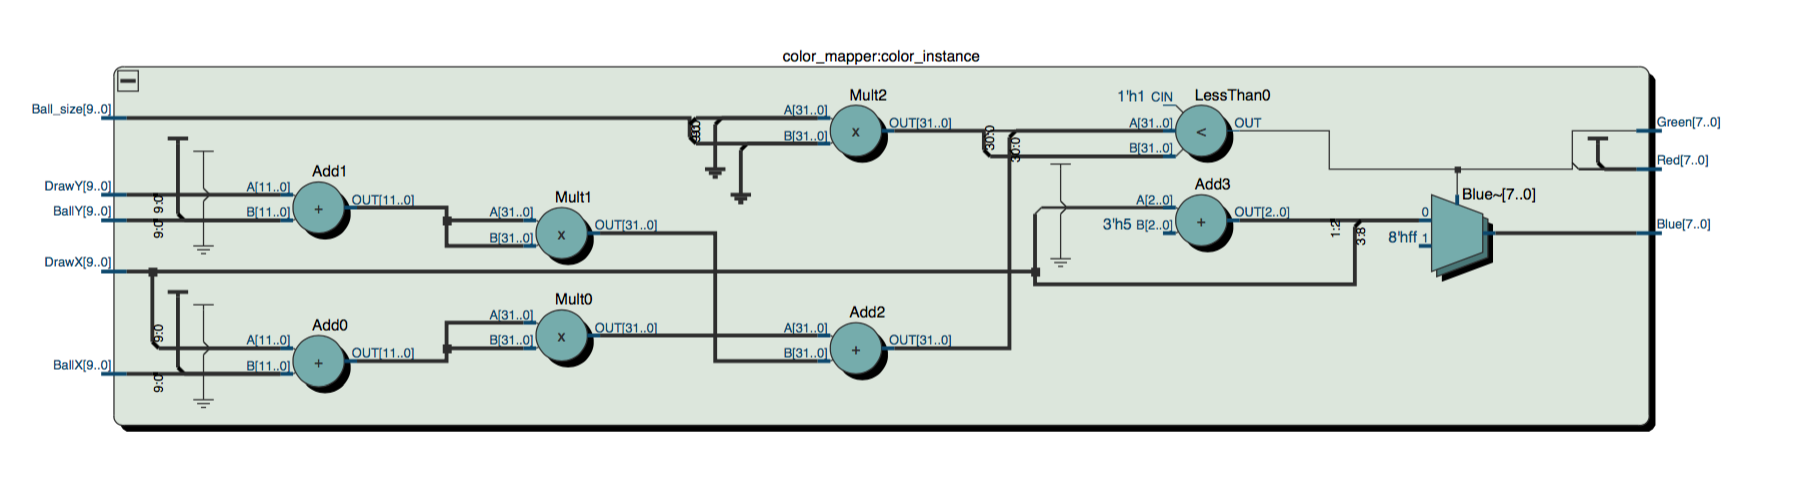
\includegraphics[scale=.5]{color_mapper_diagram.png}
%	\caption{Color Mapper Circuit Diagram\label{fig:color_mapper}}
%\end{figure}            

     

\section*{Appendix}
%\begin{lstlisting}
%void IO_write(alt_u8 Address, alt_u16 Data)
%{
%
%}
%\end{lstlisting}

\end{document}
